\setcounter{page}{0}
\chapter{\chapternameintro} \label{introduction}

As galáxias são sistemas gravitacionalmente ligados, compostos por matéria bariônica e não bariônica: estrelas, gás, poeira e matéria escura. Elas estão presentes no universo observável em diversos tamanhos e formas, desde as anãs até as gigantes. Elas são a base para a cosmologia e parte fundamental para entender a evolução do universo. São peças que reconstituem os blocos de formação do universo, e dessa forma conectam o entendimento desde as estruturas de menor escala, como nosso próprio sistema estelar, até as maiores estruturas do universo.

Nas últimas décadas, com o desenvolvimento de novos instrumentos na área observacional (e.g., \citealp{hubble_classification_1926},  \citealp{JWT_2006}, \citealp{VLT_2010}), foi possível compreender melhor os mecanismos de formação e evolução das galáxias. Com os novos levantamentos de dados, maior profundidade e melhoria na qualidade das observações, temos em mãos grandes catálogos com milhões de galáxias observadas, presentes em diversos ambientes e em diferentes épocas do universo (e.g., \citealp{SDSS_2000}, \citealp{COSMOS_2007}, \citealp{DES_2018}, \citealp{oliveira2019splus}). Além disso, houve avanços nos modelos e simulações, com melhores softwares e hardwares, possibilitando análises mais detalhadas dos dados e permitindo validar os modelos teóricos (e.g., \citealp{Vogelsberger_2014}, \citealp{EAGLE_2015}).

Uma das dificuldades que temos é modelar como as galáxias se formam ao longo do tempo, necessitando de um melhor entendimento dos processos internos em pequena e larga escala. Atualmente, acreditamos que a formação das galáxias começou a partir de pequenas flutuações no campo de densidade primordial do universo, que foram evoluindo após o início do Big Bang \citep{liddle_1999}. Assim, as estruturas do universo foram surgindo de forma hierárquica, com as galáxias mais massivas se formando a partir das menores, por meio de fusões e interações gravitacionais.

Nesta seção, falarei brevemente sobre o entendimento da formação de galáxias. Além disso, discutirei os tipos de galáxias mais massivas e, principalmente, os tipos das galáxias anãs. Nas próximas seções, tratarei sobre as propriedades e cenários de formação do objeto de interesse deste trabalho, as galáxias anãs ultra-compactas ({\it ultra compact dwarfs}, UCDs), bem como das galáxias compactas com linhas de emissão.

\section{Modelos de formação de Galáxias}\label{subsec:modelo_formacao_galaxias}
O modelo padrão cosmológico mais amplamente utilizado atualmente é o modelo $\Lambda$ Cold Dark Matter ($\Lambda CDM$), que propõe que o universo é constituído principalmente por matéria escura fria ({\it cold dark matter}, CDM) e energia escura, representada por uma constante cosmológica $\Lambda$, responsável pela expansão acelerada do universo. A designação "fria" para a matéria escura refere-se ao fato de que ela se move lentamente em comparação à velocidade da luz. 

No modelo $\Lambda CDM$, as estruturas se formam hierarquicamente, com os objetos menores sendo formados primeiro, para então se fundirem e originarem halos maiores \citep{Blumenthal_1984}.

Considerando que o universo teve início no Big Bang, expandindo-se e esfriando, as primeiras flutuações de densidade surgiram devido a flutuações quânticas no campo de densidade primordial \citep{liddle_1999}. Inicialmente, o universo era composto por um plasma quente e denso de fótons e matéria, que se expandiu e esfriou gradualmente. Com o tempo, atingiu densidades e temperaturas suficientemente baixas para permitir a formação dos primeiros átomos estáveis, principalmente hidrogênio neutro.

A radiação cósmica de fundo (CMB) é a radiação eletromagnética liberada quando o universo, já suficientemente frio para a formação de átomos, tornou-se transparente. Nesse momento, os fótons desacoplaram-se da matéria bariônica, propagando-se livremente e formando a radiação que observamos atualmente, permeando todo o universo. No modelo $\Lambda CDM$, as flutuações no campo de densidade da CMB atuam como sementes para a formação de estruturas maiores. De acordo com medições da CMB, especialmente as mais recentes, como as do \textit{Planck} \citep{Planck_2020}, o universo tem cerca de 13,8 bilhões de anos e é composto principalmente por energia escura ($\Omega_\Lambda \sim 0,7$), matéria escura ($\Omega_{DM} \sim 0,25$) e bárions ($\Omega_b \sim 0,05$).

Para descrever os eventos subsequentes de formação de galáxias até os dias atuais, considera-se a evolução em função do desvio para o vermelho (redshift, $z$).

Entre $z \sim 30$ e $z \sim 10$, os bárions conseguiram se acumular nos primeiros halos de matéria escura formados no universo, permitindo o surgimento das primeiras estrelas das galáxias (e.g., \citealp{Glover_2005}, \citealp{Greif_2015}, \citealp{Schauer_2021}). Essas primeiras estrelas, conhecidas como estrelas de população III, eram compostas apenas de hidrogênio e hélio, sendo extremamente massivas e brilhantes. A radiação emitida por essas estrelas ionizou o hidrogênio ao seu redor, e, em $z \sim 10-6$, a ionização do hidrogênio, causada por essas estrelas ou por gerações subsequentes (como a população II), marcou o fim da época da reionização \citep{Wise_2019}. Durante esse período, as galáxias começaram a se formar e evoluir, com a formação de estrelas e a evolução de suas populações estelares. Estruturas maiores, como aglomerados e superaglomerados, também começaram a se formar por meio de fusões e interações gravitacionais. Sob a influência gravitacional, essas estruturas evoluem e se fundem, formando a teia cósmica em larga escala.

No contexto do modelo $\Lambda CDM$, a formação de galáxias ocorre de forma hierárquica. Simulações cosmológicas que incorporam dissipação de gás e física bariônica, juntamente com a matéria escura, sugerem um esquema de formação em duas fases (e.g., \citealp{Oser_2010}, \citealp{Pillepich_2014}). Na primeira fase, as estrelas formam-se na própria galáxia a partir do gás presente no halo de matéria escura. Na segunda fase, a galáxia cresce ao incorporar galáxias satélites por meio de fusões. Na Via Láctea, por exemplo, observa-se esse crescimento por fusões, evidenciado pelas galáxias satélites que estão sendo incorporadas ou pelas estrelas de correntes mareais deixadas por essas fusões. As correntes mareais consistem em estrelas que foram arrancadas de galáxias menores, que foram incorporadas pela galáxia principal. Um exemplo notável na Via Láctea é a corrente de Sagitário, deixada pela galáxia anã de Sagitário, que está sendo incorporada pela nossa galáxia \citep{Law_2016}.

Nas galáxias mais distantes, a observação dessas correntes é mais desafiadora devido ao seu baixo brilho superficial. No entanto, para galáxias externas, as melhores evidências de fusões moldando galáxias vêm de sistemas atualmente interagindo, que frequentemente apresentam morfologias e cinemáticas perturbadas.

Em escalas maiores, a teia cósmica, composta por filamentos, vazios e nós, é uma das principais estruturas observadas. Os filamentos, formados por matéria escura e galáxias, conectam os nós, que são aglomerados de galáxias massivos. Entre os filamentos, encontram-se os vazios, regiões de baixa densidade de matéria e galáxias \citep{Lindner_1995}. Observações recentes permitiram mapear a distribuição de galáxias e reconstruir a teia cósmica (\citealp{Lindner_1995}, \citealp{Abazajian_2003}), cujas propriedades estão, em geral, de acordo com os resultados de simulações cosmológicas, representando um dos grandes sucessos do modelo $\Lambda CDM$.

Apesar do sucesso do modelo $\Lambda CDM$, ainda existem desafios e teorias alternativas propostas. As naturezas da matéria escura e da energia escura permanecem desconhecidas, e há inconsistências em escalas pequenas e grandes. Um exemplo é o problema dos satélites ausentes na Via Láctea (\citealp{Klypin_1999}, \citealp{Moore_1999}). Embora o número de satélites observados tenha aumentado com novos estudos, ainda há uma discrepância em relação ao número previsto por simulações. Não está claro se essa diferença é real ou se decorre da não detecção de halos ainda não observados. A ausência de pequenas estruturas implica que a formação de galáxias ocorre em subhalos da Via Láctea, mas essas estruturas são menos densas do que o esperado em simulações \citep{Boylan_Kolchin_2011}. Essas dificuldades levaram à consideração de cenários cosmológicos alternativos, como inflação não padrão (e.g., \citealp{Kamionkowski_2000}) ou matéria escura não fria (e.g., \citealp{Murgia_2017}). No entanto, o modelo $\Lambda CDM$ continua sendo o mais aceito e bem-sucedido para explicar a formação e evolução do universo, reproduzindo com precisão observações em escalas maiores que alguns quiloparsecs.

\subsection{Galáxias Early e Late - type}\label{subsec:Galaxia_early_late}
Em 1926, Edwin Hubble criou um dos primeiros esquemas para a classificação de galáxias, dividindo-as em categorias que abrangiam os objetos mais luminosos e massivos: galáxias elípticas, lenticulares e espirais \citep{hubble_classification_1926}. As galáxias elípticas são caracterizadas por sua forma esferoidal e, de forma geral, cessaram sua formação estelar, possuindo uma população estelar mais velha e com menos gás e poeira. Juntamente com as lenticulares (S0), que diferem das elípticas por terem um disco de estrelas e poeira, mas sem a presença de braços espirais, são conhecidas como galáxias early-type.

Já as espirais são caracterizadas por terem um disco de estrelas, gás e poeira, com braços espirais e um bojo central, e são conhecidas como galáxias late-type. Na Figura \ref{hubble_sequence}, é possível observar a sequência de Hubble, que mostra a classificação de galáxias de acordo com sua morfologia. Na Figura \ref{galaxies_morphology}, é possível ver exemplos de galáxias de diferentes tipos morfológicos, na mesma ordem apresentada na Figura \ref{hubble_sequence}, para exemplos de galáxias \textit{E0}, \textit{S0} e \textit{Irregular}. Fora desse esquema de classificação, temos as galáxias de baixa massa, que apresentam morfologias mais irregulares.

\begin{figure}[!ht]
    \begin{center}
    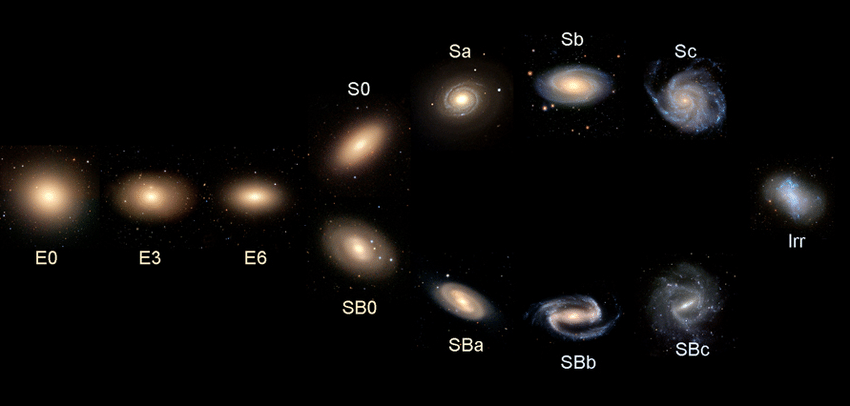
\includegraphics[width=0.7\columnwidth,angle=0]{indroduction/hubble_sequence.png}
    \caption[]{Sequência de Hubble, mostrando a classificação de galáxias de acordo com a morfologia. Créditos: \cite{huble_sequence_img}.}
    \label{hubble_sequence}
    \end{center}
\end{figure}


\begin{figure}[!ht]
    \centering
    \captionsetup{justification=centering}
    \begin{subfigure}[b]{0.237\textwidth}
        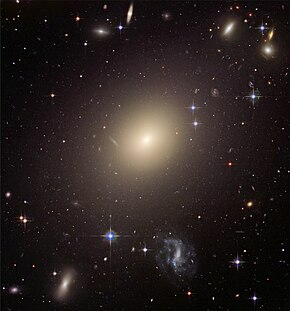
\includegraphics[width=\textwidth]{indroduction/E0_ex.png}
        \caption{}
    \end{subfigure}
    \begin{subfigure}[b]{0.26\textwidth}
        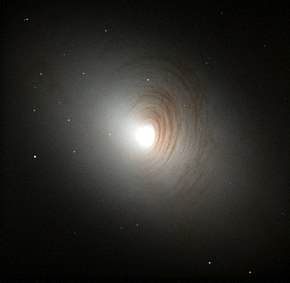
\includegraphics[width=\textwidth]{indroduction/S0_ex.png}
        \caption{}
    \end{subfigure}
    \begin{subfigure}[b]{0.268\textwidth}
        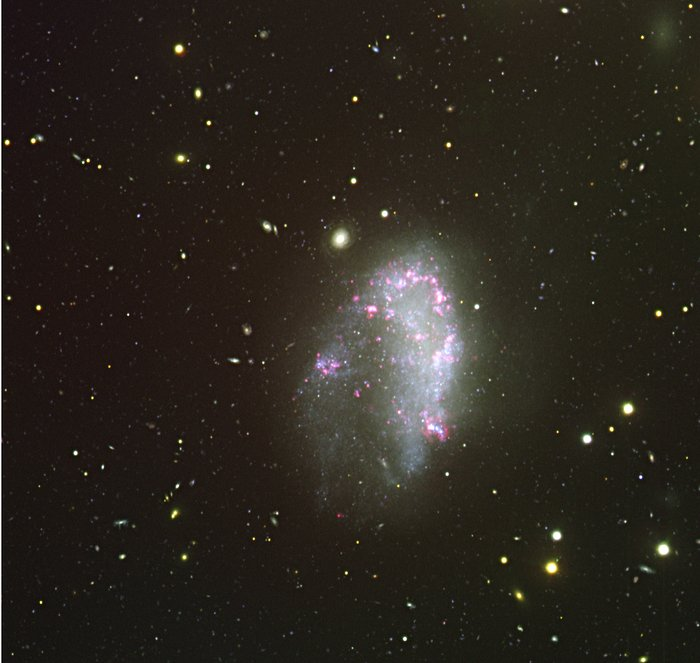
\includegraphics[width=\textwidth]{indroduction/irregular_ex.png}
        \caption{}
    \end{subfigure}
    \caption{Exemplos de diferentes tipos morfologios de galáxias. a) Early-type (E0) ESO 325-4, b) Lenticular (S0) NGC 2787, c) Irregular NGC 1427. Créditos: a) NASA/ESA, b) NASA/ESA, c) ESO.}
    \label{galaxies_morphology}
\end{figure}

\subsection{Galáxias anãs}\label{subsec:dwarf_galaxies}
As galáxias anãs estão presentes no universo em uma ampla variedade de formas, com diferentes tipos de estruturas e composições. Elas representam a categoria mais numerosa de galáxias no universo. Esse tipo de galáxia é caracterizado por sua baixa luminosidade, como o próprio nome sugere, sendo significativamente menos luminosas e menores do que suas contrapartes maiores.

O limite exato para categorizá-las em termos de luminosidade, por exemplo, é incerto e não é uniformemente definido. Suas massas geralmente variam entre $10^5$ e $10^9$ massas solares. Inicialmente, os critérios de classificação das galáxias anãs baseavam-se em características observacionais, como suas morfologias e brilho superficial \citep{dwarf_classification_init}. No entanto, com os avanços nos dados observacionais, que anteriormente eram limitados para sistemas menores e mais fracos, surgiram novos critérios que consideram propriedades como a cinemática interna. Além disso, a distinção entre os tipos de galáxias anãs também pode ser feita com base no meio interestelar, utilizando a presença de gás e poeira como critério.

No caso das galáxias anãs com pouca quantidade de gás, essa característica pode ser atribuída, em parte, às interações com galáxias maiores, que podem remover o gás dessas galáxias, impedindo a formação de novas estrelas. Além disso, a pressão de radiação e os ventos estelares provenientes de estrelas massivas podem expelir o gás das galáxias anãs, dificultando a retenção de gás no meio interestelar. Outro mecanismo relevante é a remoção de gás por pressão de arrasto (\textit{ram pressure stripping}), que ocorre quando uma galáxia anã se move através do meio intraaglomerado quente e denso de um aglomerado de galáxias. Essa interação pode remover o gás interestelar, especialmente em regiões periféricas, reduzindo ainda mais a capacidade dessas galáxias de formar novas estrelas.

As galáxias anãs de menor massa pertencem a esse grupo e, devido às suas baixas luminosidades, foram inicialmente identificadas nas regiões mais próximas, como no Grupo Local. Elas podem ser divididas em dois principais grupos: as galáxias anãs esferoidais (\ac{dSph}) e as galáxias anãs elípticas (\ac{dE}). As anãs elípticas, que são as mais massivas desse grupo, foram observadas em aglomerados de galáxias e inicialmente classificadas como uma categoria separada de galáxias mais massivas, apresentando características distintas de suas contrapartes locais. No entanto, estudos como o de \cite{Forbes_2011} sugeriram uma transição contínua entre os tipos \ac{dSph} e \ac{dE}.

Entre as galáxias anãs com maior conteúdo de gás, destacam-se as anãs compactas azuis (\ac{BCD}) e as anãs irregulares (\ac{dIrr}). As BCDs também são conhecidas por outros nomes na literatura, como galáxias H II, devido à semelhança de seus espectros com regiões H II, e '\textit{green peas}', uma classe de galáxias compactas e intensamente formadoras de estrelas. Devido à presença de gás, essas galáxias apresentam formação estelar contínua. No caso das BCDs, a formação estelar ocorre em surtos intensos, mas de curta duração, enquanto as dIrrs apresentam formação estelar prolongada, embora em taxas mais baixas \citep{McQuinn2010}.

Dentro do grupo de galáxias anãs de baixa massa e luminosidade, temos as galáxias ultra-difusas (UDG). Por serem extremamente difusas, seus tamanhos podem ser comparáveis aos de algumas galáxias massivas, embora suas massas sejam muito baixas, em torno de $10^7$ massas solares \citep{van_Dokkum2015}.

Devido à sua natureza difusa, baixa massa e baixa luminosidade, as UDGs são extremamente difíceis de detectar e observar. Como um dos extremos no espectro de massas das galáxias, elas representam um desafio para o modelo padrão e podem fornecer insights valiosos sobre a formação e evolução de galáxias, bem como sobre a distribuição da matéria escura.

Por fim, temos as galáxias anãs ultra-compactas (UCDs), que são o foco deste trabalho na busca por novos objetos. Na próxima seção, discutiremos as UCDs em maior detalhe, abordando sua origem, localização, cenários de formação e propriedades, além de explorar como elas se correlacionam com outro tipo de objeto conhecido como aglomerados estelares nucleares (NSC).

A Figura \ref{dwarf_galaxies} apresenta exemplos de galáxias anãs de diferentes tipos morfológicos: a primeira imagem mostra uma galáxia anã esferoidal (\ac{dSph}), a segunda uma galáxia anã elíptica (\ac{dE}), a terceira uma galáxia anã irregular (\ac{dIrr}) e a quarta uma galáxia anã compacta azul (\ac{BCD}).

\begin{figure}[!ht]
    \centering
    \captionsetup{justification=centering}
    \begin{subfigure}[b]{0.33\textwidth}
        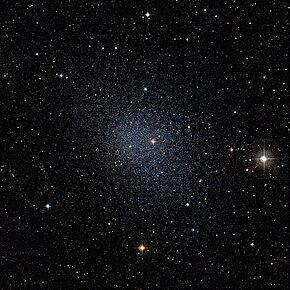
\includegraphics[width=\textwidth]{indroduction/dSph.png}
        \caption{}
    \end{subfigure}
    \begin{subfigure}[b]{0.33\textwidth}
        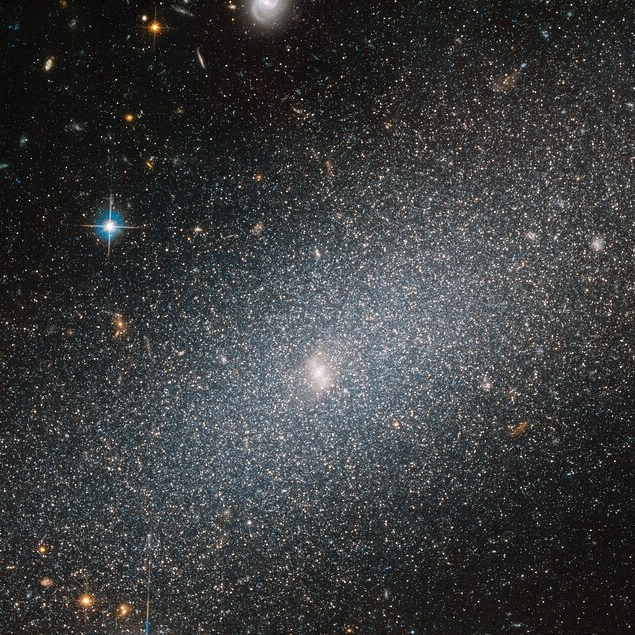
\includegraphics[width=\textwidth]{indroduction/dE.png}
        \caption{}
    \end{subfigure}
    \begin{subfigure}[b]{0.33\textwidth}
        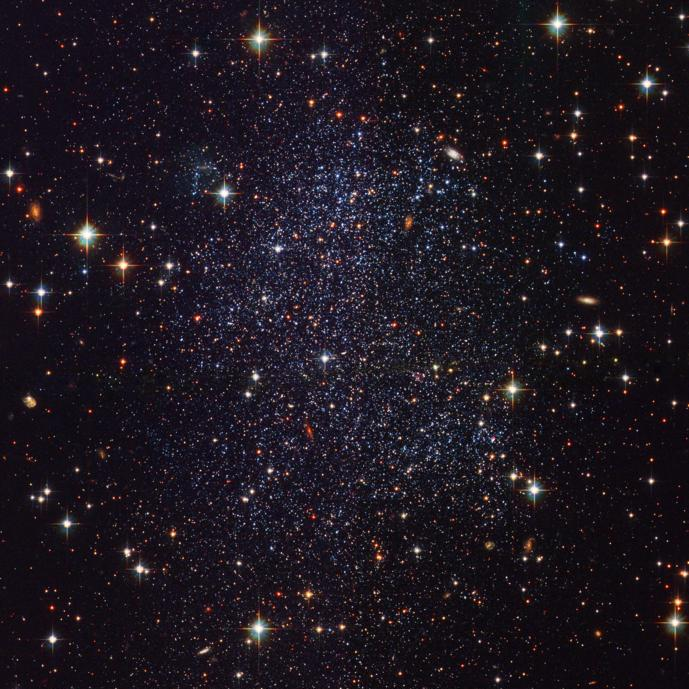
\includegraphics[width=\textwidth]{indroduction/dIrr.png}
        \caption{}
    \end{subfigure}
    \begin{subfigure}[b]{0.33\textwidth}
        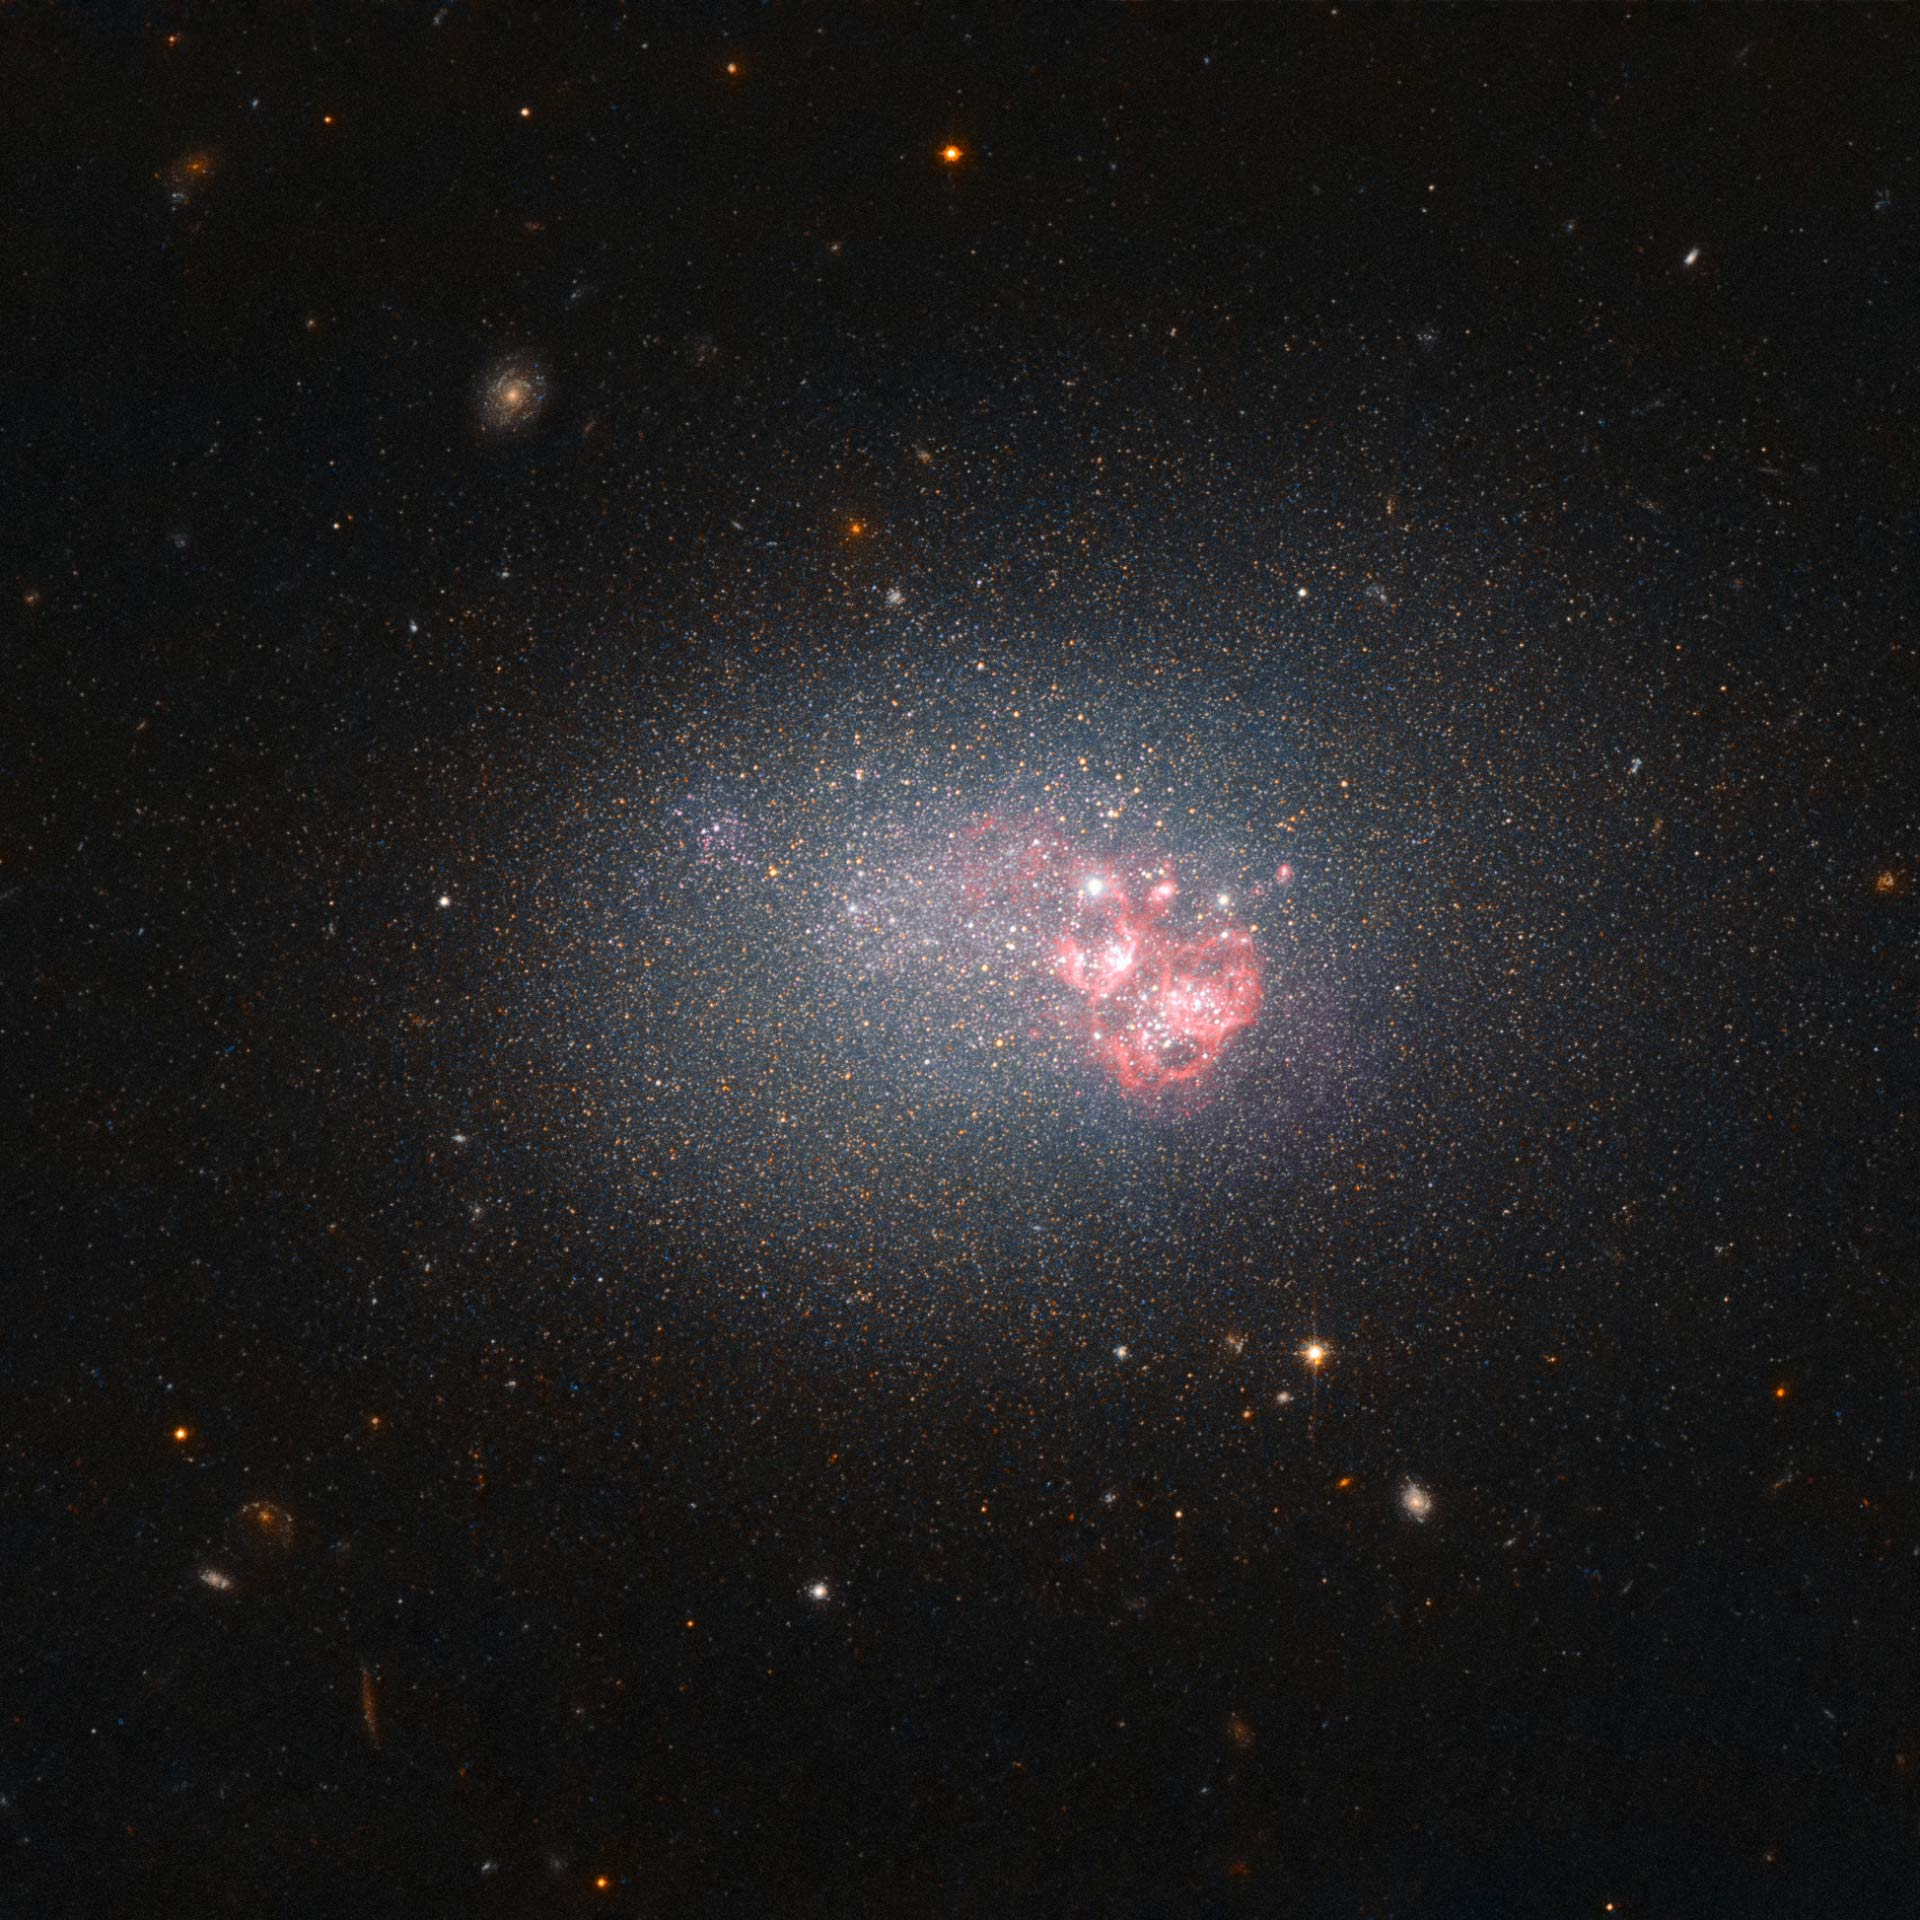
\includegraphics[width=\textwidth]{indroduction/BCD.png}
        \caption{}
    \end{subfigure}
    \caption{Exemplos de diferentes tipos morfologios de galáxias anãs conhecidas. a) Anã esferoidal (dSph) Fornax Dwarf Spheroidal, b) Anã elíptica (dE) PGC 29388, c) Anã irregular (dIrr) SagDIG, d) Anã compacta azul (BCD) LEDA 17302. Créditos: a) ESO/Digitized Sky Survey 2, b) ESA/Hubble, c)NASA, ESA, and The Hubble Heritage Team (STScI/AURA), d) NASA/ESA/Hubble.}
    \label{dwarf_galaxies}
\end{figure}

\section{As galáxias anãs ultra-compactas (UCDs)}\label{sec:UCDs}
As galáxias anãs ultra-compactas (UCDs) formam uma classe de objetos que se posiciona entre as galáxias anãs e os aglomerados globulares (\ac{GC}). Elas foram inicialmente descobertas em levantamentos espectroscópicos no aglomerado de Fornax por \cite{Drinkwater_2000} e \cite{Hilker_1999}. Desde então, passaram a ser identificadas em outros aglomerados e grupos de galáxias próximos, como Virgo (\citealp{Hasegan_2005}; \citealp{Liu_2020}), Abell 1689 \citep{Mieske_2005}, Centaurus \citep{Mieske_2007}, Hydra \citep{Wehner_Harris_2007}, Abell S0740 \citep{Blakeslee_DeGraaff2008}, no grupo NGC 1023 \citep{Mieske_West_Oliveira_2007}, no Grupo Dorado \citep{Evstigneeva_2007}, no grupo NGC 5044 \citep{Faifer_2017}, no grupo NGC 3613 \citep{Bortoli_2020} e no grupo fóssil NGC 1132 \citep{Madrid_2011}. Além disso, UCDs também foram encontradas ao redor de galáxias isoladas \citep{Hau_2009}.

Até o final dos anos 2000, acreditava-se que as divisões entre sistemas classificados como aglomerados estelares e galáxias eram mais rígidas. Devido às controvérsias sobre suas origens, as UCDs já foram denominadas objetos ultracompactos (UCOs) \citep{Mieske_2002} e objetos de transição globular-anã (DGTOs) \citep{Hasegan_2005}. Tradicionalmente, as galáxias eram categorizadas pela presença de matéria escura e por tamanhos superiores a alguns quiloparsecs, enquanto os aglomerados estelares eram considerados conjuntos de estrelas com raios de poucos parsecs, sem a presença de matéria escura. No entanto, com a descoberta das UCDs, essa distinção tornou-se mais complexa, pois elas apresentam características de ambos os grupos, sendo inicialmente classificadas como objetos intermediários.

Apesar do aumento no número de UCDs descobertas e dos avanços em estudos que investigam sua origem, evolução e propriedades, o processo de formação dessas galáxias permanece controverso. Os cenários de formação das UCDs serão discutidos em maior detalhe na seção \ref{subsec:formacao}. De forma resumida, as principais teorias seguem duas linhas: (1) a formação de UCDs a partir de galáxias anãs nucleadas que sofreram processos de despojamento gravitacional (\textit{stripping}) e (2) a formação de UCDs a partir de aglomerados globulares massivos. Contudo, as evidências indicam que nenhum desses cenários, isoladamente, é capaz de explicar todas as populações conhecidas de UCDs. Assim, uma combinação de processos, envolvendo múltiplos canais de formação, parece ser a solução mais plausível para explicar a diversidade de propriedades observadas nesses objetos.

Mostramos na Figura \ref{UCDs_exp} exemplos de galáxias anãs ultra-compactas encontradas em diferentes ambientes, sendo a primeira imagem uma UCD encontrada próxima a M60, a segunda uma UCD encontrada próxima a M87 e a terceira uma UCD encontrada próxima a NGC 1399, no aglomerado de Fornax.

\begin{figure}[!ht]
    \centering
    \captionsetup{justification=centering}
    \begin{subfigure}[b]{0.3\textwidth}
        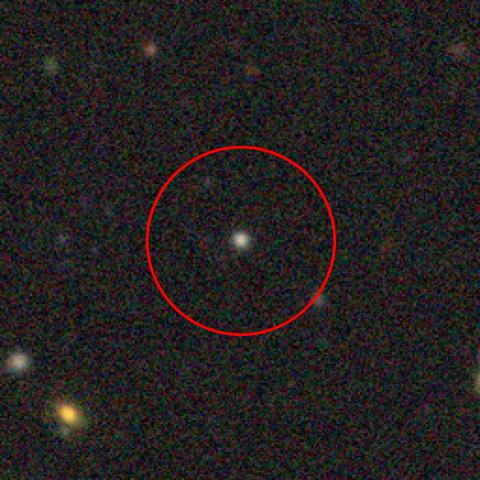
\includegraphics[width=\textwidth]{Images/ucds_exp/UCD_M60.png}
        \caption{}
    \end{subfigure}
    \begin{subfigure}[b]{0.3\textwidth}
        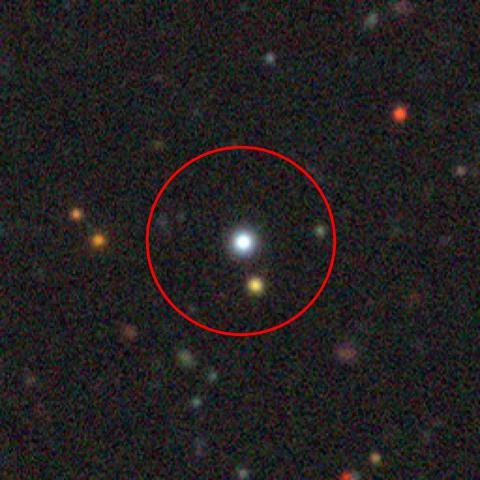
\includegraphics[width=\textwidth]{Images/ucds_exp/UCD_M87.png}
        \caption{}
    \end{subfigure}
    \begin{subfigure}[b]{0.3\textwidth}
        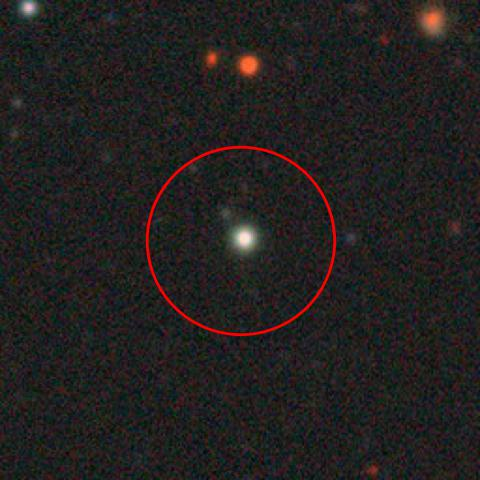
\includegraphics[width=\textwidth]{Images/ucds_exp/UCD_NGC1399.png}
        \caption{}
    \end{subfigure}
    \caption{Exemplos de galáxias anãs ultra-compactas encontradas em diferentes ambientes. a) UCD - galáxia hospedeira M60, b) UCD - galáxia hospedeira M87, c) UCD - galáxia hospedeira NGC 1399. Créditos: a) Legacy Survey, b) Legacy Survey, c) Legacy Survey.}
    \label{UCDs_exp}
\end{figure}

\subsection{Propriedades das UCDs}\label{subsec:propriedade}
Quando comparadas a aglomerados globulares típicos, as UCDs são maiores, mais brilhantes e mais massivas. Seus raios de meia-luz variam entre 7 e 100 parsecs ($7 \leq r_h \leq 100$ pc) \citep{Mieske_2008_1}, enquanto suas luminosidades situam-se na faixa de $-14 \leq M_g \leq -10$ magnitudes, considerando a magnitude absoluta na banda $V$ \citep{Voggel_2016}.

As massas das UCDs variam entre $10^6$ e $10^8$ massas solares ($M_{\odot}$) (\citealp{Mieske_2008_1}; \citealp{Misgeld_2011_2}), sendo o limite inferior adotado como critério para diferenciá-las de aglomerados estelares massivos. Essa distinção baseia-se em dois fatores principais: primeiro, sistemas estelares compactos começam a exibir uma relação tamanho-luminosidade acima dessa massa (\citealp{Hasegan_2005}; \citealp{Cote_2006}; \citealp{Rejkuba_2007}; \citealp{Evstigneeva_2008}; \citealp{Norris_2011}), o que os diferencia de aglomerados globulares, cujos tamanhos são independentes da luminosidade \citep{Jornan_2005}. Em segundo lugar, a razão massa-luminosidade ($M/L$) dos sistemas estelares compactos aumenta significativamente acima de $10^6$ $M_{\odot}$, excedendo os valores previstos por modelos de populações estelares com funções de massa iniciais (IMFs) canônicas (\citealp{Hasegan_2005}; \citealp{Dabringhausen_2008}).

As UCDs apresentam predominantemente populações estelares antigas, com uma ampla gama de metalicidades (\citealp{Evstigneeva_2009}; \citealp{Janz_2015}; \citealp{Zhang_2018}; \citealp{Forbes_2020}; \citealp{Fahrion_2020}). Suas dispersões de velocidade central variam entre $20 < \sigma_0 < 50$ km s$^{-1}$ (\citealp{Hasegan_2005}; \citealp{Mieske_2008_1}), sendo a relação $M-\sigma_0$ consistente com a relação Faber-Jackson para galáxias elípticas.

Além disso, as UCDs possuem, em média, uma razão de massa dinâmica para massa estelar de $M_{dyn}/M_* > 1$ ($M_{dyn}/M_* = 1.7 \pm 0.2$ para UCDs massivas, com $M > 10^7 M_{\odot}$), enquanto para aglomerados globulares típicos, $M_{dyn}/M_* \approx 1$ \citep{Mieske_2013}.

A razão massa-luminosidade ($M/L$) das UCDs tem sido amplamente investigada na literatura (\citealp{Hasegan_2005}; \citealp{Dabringhausen_2009}, \citeyear{Dabringhausen_2010}, \citeyear{Dabringhausen_2012}; \citealp{Baumgardt_2008}; \citealp{Mieske_2008_2}; \citealp{Taylor_2010}; \citealp{Frank_2011}; \citealp{Strader_2013}). Observações indicam que, especialmente nas UCDs mais massivas, os valores de $M/L$ podem ser até 50\% maiores do que os previstos por modelos de populações estelares com IMFs canônicas (\citealp{Hasegan_2005}; \citealp{Mieske_2008_2}). Comparadas a aglomerados globulares de metalicidades semelhantes, as UCDs podem apresentar razões $M/L$ até duas vezes maiores, particularmente na banda $V$.

Essa elevação na razão $M/L$ tem sido proposta como um critério para distinguir UCDs de aglomerados globulares. No entanto, a origem dessa elevação ainda é incerta. Por exemplo, \cite{Voggel_2018} sugerem que a quantidade de UCDs com $M/L$ elevado pode estar superestimada devido a limitações observacionais e modelagens anteriores.

As explicações para os valores elevados de $M/L$ nas UCDs são diversas e podem ser atribuídas a uma combinação de fatores. As principais hipóteses incluem a presença de matéria escura, variações na Função Inicial de Massa (IMF), a presença de buracos negros supermassivos ou perturbações causadas pela proximidade de galáxias massivas. Assim como os cenários de formação das UCDs, a razão elevada de $M/L$ parece depender de múltiplos fatores, refletindo a complexidade desses sistemas.

\subsection{Cenários de Formação das UCDs}\label{subsec:formacao}
Os cenários de formação das galáxias anãs ultra-compactas ainda são amplamente debatidos, com diversas teorias propostas para explicar sua origem. As hipóteses mais aceitas seguem duas linhas principais: a primeira sugere que as UCDs são remanescentes de galáxias anãs nucleadas que foram despojadas de suas camadas externas devido a interações gravitacionais com galáxias maiores em ambientes densos, como aglomerados de galáxias. Nesse contexto, o termo "despojada" refere-se ao processo de remoção das regiões externas da galáxia, deixando apenas o núcleo compacto. A segunda linha sugere que as UCDs se formaram a partir de aglomerados estelares massivos. O consenso atual é que as UCDs pertencem a uma família de objetos cuja origem pode ser explicada por múltiplos cenários.

Dentro dessas linhas de pensamento, há a proposta de que as UCDs podem resultar da fusão de aglomerados estelares (\citealp{Kroupa_1998}; \citealp{Fellhauer_2002}; \citealp{Br_ns_2012}) ou surgir diretamente como aglomerados globulares extremamente massivos, formados em sistemas ricos em tais objetos (\citealp{Mieske_2002}; \citealp{Mieske_2011}). Por outro lado, no cenário de galáxias despojadas, as UCDs seriam formadas a partir de núcleos remanescentes de galáxias anãs que sofreram interações gravitacionais intensas, resultando na remoção de suas regiões externas e deixando apenas o núcleo compacto como o objeto final (\citealp{Bassino_1994}; \citealp{Bekki_2001}; \citealp{Drinkwater_2003}; \citealp{Goerdt_2008}; \citealp{Pfeffer_2013}).

Nas próximas subseções, exploraremos essas linhas de evolução em maior detalhe, destacando os principais mecanismos e evidências que sustentam cada cenário.

\subsubsection{Aglomerados globulares (GC)}\label{subsubsec:}
No contexto da origem das UCDs como aglomerados estelares, sugere-se que elas possam ser aglomerados globulares extremamente massivos e luminosos, formados em regiões próximas a galáxias com sistemas ricos em tais objetos \citep{Mieske_2002}.

Uma possibilidade é que as UCDs surjam a partir da fusão de aglomerados globulares em regiões de alta densidade \citep{Fellhauer_2002}. Simulações que investigam as possíveis origens por meio da fusão de múltiplos aglomerados globulares \citep{Goerdt_2008} demonstram que é possível reproduzir as propriedades observadas nas UCDs, como suas massas, tamanhos e luminosidades. Estima-se que sejam necessários cerca de 50 aglomerados globulares para formar objetos com características semelhantes às UCDs \citep{Goerdt_2008}.

Estudos comparativos da razão massa-luminosidade ($M/L$) na banda $V$ com modelos de populações estelares indicaram compatibilidade para UCDs nos aglomerados de Fornax \citep{Hilker_2006} e Virgo \citep{Evstigneeva_2007}. Em uma análise detalhada de uma das primeiras UCDs descobertas, a \textit{UCD3} no aglomerado de Fornax, \cite{Frank_2011} não encontrou evidências convincentes de matéria escura ou de um buraco negro central que pudesse justificar um aumento na razão $M/L$. A dinâmica interna observada foi consistente com a de um aglomerado estelar massivo, reforçando a hipótese de que algumas UCDs podem se originar de aglomerados estelares.

\subsubsection{Despojamento de galáxias}\label{subsubsec:Galaxy stripping}
Na linha de raciocínio sobre a origem das UCDs, uma das hipóteses mais estudadas é sua formação a partir de interações gravitacionais que despojam as regiões externas de galáxias nucleadas, resultando em objetos compactos.

Uma galáxia nucleada, após passar por fusões e interações gravitacionais, pode ter seu núcleo central preservado, permanecendo como um aglomerado luminoso \citep{Bassino_1994}. Exemplos apresentados por \cite{Bekki_2001} mostram que, mesmo após múltiplas passagens da galáxia original pela região central de um aglomerado, as regiões externas são removidas, enquanto o núcleo permanece relativamente intacto, resultando em um objeto final com características semelhantes às UCDs.

Ao comparar as distribuições observadas de UCDs em aglomerados com as previsões de modelos de formação, como os de \cite{Thomas_2008}, observa-se uma boa correspondência em regiões centrais. No entanto, esses modelos preveem uma maior produção de UCDs em raios maiores, o que não é confirmado pelos dados observacionais. Essa discrepância pode ser atribuída ao fato de que os modelos estáticos não consideram mudanças dinâmicas ao longo da evolução dos aglomerados, como fusões de subestruturas ou outras interações gravitacionais, que podem influenciar a distribuição radial das UCDs.

De acordo com \cite{Bekki_2003}, o tempo necessário para que essas interações ocorram e formem UCDs é da ordem de bilhões de anos. As órbitas envolvidas precisam ser altamente excêntricas, e a galáxia hospedeira deve ser mais luminosa do que $M_B = -16$. Tanto órbitas elípticas, com múltiplas aproximações próximas da galáxia original, quanto órbitas mais caóticas, com poucas aproximações, podem levar à formação de UCDs. Esses cenários produzem objetos com variações em luminosidade e tamanho, dependendo das características das interações, explicando a diversidade observada nas UCDs.

Após o processo de despojamento, o núcleo da galáxia anã sofre uma expansão moderada, aumentando seu tamanho efetivo em cerca de 2 a 3 vezes em relação ao tamanho original. Esse aumento é consistente com as observações de \cite{Evstigneeva_2008}, que indicam que as UCDs possuem raios efetivos aproximadamente duas vezes maiores do que os núcleos de galáxias anãs elípticas (dE) de luminosidade similar.

Estudos de \cite{Pfeffer_2016} investigaram as contribuições dos núcleos despojados na formação das UCDs e previram que o número de núcleos despojados escala com a massa virial do hospedeiro. Eles sugerem que as UCDs de alta massa representam um grupo misto de objetos formados por diferentes processos, enquanto as UCDs de menor massa provavelmente se originam de aglomerados globulares.

Além disso, \cite{Pfeffer_2016} analisaram as metalicidades das galáxias progenitoras de núcleos despojados e compararam com as metalicidades observadas em aglomerados globulares e UCDs. Eles concluíram que há uma boa concordância entre as metalicidades de UCDs e núcleos despojados para objetos com massa $M > 5 \times 10^6 M_{\odot}$.

Para aprimorar a comparação entre esses cenários, ainda existem desafios a serem superados, como as limitações de resolução em modelos semianalíticos e a ausência de uma descrição detalhada da componente bariônica. A componente bariônica influencia tanto o tempo necessário para o despojamento das galáxias quanto o número de galáxias que passam por esse processo. Nesse contexto, simulações hidrodinâmicas cosmológicas são essenciais para obter resultados mais precisos. No entanto, a baixa resolução dessas simulações para galáxias anãs e de menor massa ainda representa uma dificuldade. Além disso, é crucial compreender melhor como os tempos e taxas de fusão evoluem em altos redshifts para aprimorar os modelos de formação de UCDs.

\subsubsection{Aglomerados estelares nucleares (NSCs)}\label{subsubsection:NSC}
Sobre a origem e os cenários de formação das UCDs, discutidos no início desta seção, considera-se a possibilidade de que esses objetos tenham se originado a partir de galáxias nucleadas. Vamos explorar mais detalhadamente as características desses núcleos.

Os núcleos estão associados ao que é conhecido como \ac{NSC} (Aglomerados Estelares Nucleares). Esses objetos são compactos, massivos e mais luminosos quando comparados aos aglomerados globulares. Enquanto os aglomerados globulares possuem massas na faixa de $10^4$ a $10^6 M_{\odot}$ \citep{Masters_2010}, os NSCs apresentam massas significativamente maiores, variando de $10^6$ a $10^8 M_{\odot}$ (\citealp{Spengler_2017}; \citealp{Georgiev_2016}).

Inicialmente, a detecção dos NSCs era dificultada pelas limitações das resoluções observacionais. No entanto, com o avanço de instrumentos mais eficientes, como CCDs de alta sensibilidade, tornou-se possível detectar e separar esses núcleos de maneira mais clara, identificando-os tanto em galáxias do tipo early quanto late (\citealp{Phillips_1996}; \citealp{Carollo_1997}; \citealp{Matthews_1999}; \citealp{boker_2002}).

As propriedades dos NSCs mostram correlações significativas com as características de suas galáxias hospedeiras (\citealp{Balcells_2003}; \citealp{Graham_2003}). Estudos estabeleceram relações entre a massa dos NSCs e propriedades como a luminosidade do bojo, a dispersão de velocidade e a massa estelar total da galáxia \citep{Ferrarese_2006, Wehner_2006, Rossa_2006}. Além disso, foi sugerido que os buracos negros supermassivos (SMBHs) e os NSCs seguem relações de escala semelhantes \citep{Ferrarese_2006}.

A fração de nucleação, definida como a proporção de galáxias que possuem um NSC em relação ao número total de galáxias em uma amostra, é alta. Segundo \cite{Boker_2010}, NSCs estão presentes nos centros de mais de 70\% de todas as galáxias. No caso específico das galáxias anãs, \cite{Sanchez_2019} analisaram galáxias no aglomerado de Virgo e concluíram que a fração de nucleação atinge um máximo de 90\% para galáxias com massas $M_{gal} \approx 10^9 M_{\odot}$, diminuindo para menos de 10\% em galáxias com massas muito altas ($M_{gal} > 10^{11} M_{\odot}$) ou muito baixas ($M_{gal} < 10^6 M_{\odot}$).

Para galáxias anãs menos massivas ($M_{gal} < 10^6 M_{\odot}$), a fração de nucleação é próxima de zero \citep{Ordenes_2018}. Além disso, essas galáxias possuem poucos aglomerados globulares (GCs) \citep{Forbes_2018}, sugerindo que não são capazes de formar aglomerados estelares massivos. Por outro lado, em galáxias anãs mais massivas, interações entre NSCs e SMBHs centrais podem levar à destruição dos NSCs existentes ou inibir a formação de novos (\citealp{Cote_2006}; \citealp{Neumayer_2012}; \citealp{Antonini_2015}; \citealp{Arca_2016}).

Casos em que SMBHs coexistem com NSCs foram identificados \citep{Graham_2009}. A fração de massa entre o SMBH e o NSC aumenta com a massa da galáxia, de modo que, em galáxias mais massivas ($M_{gal} > 3 \times 10^{10} M_{\odot}$), os SMBHs dominam a massa central. Esses sistemas podem ser influenciados por fusões binárias de buracos negros e interações dinâmicas com as estrelas do NSC \citep{Antonini_2015}. Em galáxias menores, no entanto, a massa do NSC predomina.

Estudos recentes têm explorado a continuidade evolutiva de galáxias nucleadas e sistemas ultra-compactos. Por exemplo, \cite{Wang_2023} investigaram galáxias no aglomerado de Virgo e identificaram uma sequência morfológica que conecta galáxias anãs nucleadas a UCDs. Eles sugerem que essas classes representam diferentes estágios do processo de despojamento.

\noindent A sequência evolutiva sugerida é composta por:

\begin{itemize}
    \item \textbf{Galáxias anãs elípticas nucleadas (dE,N)} – São galáxias anãs elípticas que contêm um núcleo estelar proeminente. Algumas apresentam uma fração de luminosidade nuclear significativamente alta, sendo chamadas de fortemente nucleadas.
    \item \textbf{Galáxias anãs elípticas nucleadas com envelopes estendidos (eUCDs, extended Ultra-Compact Dwarfs)} – Representam uma fase intermediária entre as dE,N e as UCDs. Esses objetos ainda retêm envelopes estelares detectáveis, embora mais compactos.
    \item \textbf{Galáxias anãs ultra-compactas (UCDs)} – Objetos extremamente compactos, com raios de meia-luz entre 10 e 100 parsecs. Muitos deles são interpretados como núcleos remanescentes de galáxias anãs que perderam a maior parte de sua massa estelar original devido à interação gravitacional com galáxias massivas.
\end{itemize}


A Figura \ref{continuo_evolution_dwarf} ilustra os diferentes tipos de galáxias discutidos por \cite{Wang_2023}, os quais representam um contínuo evolutivo esperado para sistemas que passaram pelo processo de despojamento. Esse processo pode transformar galáxias anãs nucleadas em objetos ultra-compactos, como as UCDs. Da esquerda para a direita, observamos:

\begin{itemize}
    \item Uma galáxia anã com um aglomerado estelar nuclear (NSC) bem definido;
    \item Uma galáxia ainda nucleada, mas com seu envoltório externo mostrando evidências de perturbação gravitacional por interações com galáxias massivas;
    \item Uma galáxia classificada como ultra-difusa (\ac{UDG}), com um núcleo estelar visível, embora envolvido por um envelope muito difuso e de baixa luminosidade superficial;
    \item Uma galáxia fortemente nucleada, definida por uma fração de luminosidade do núcleo significativamente alta em relação ao restante da galáxia;
    \item Por fim, dois objetos classificados como UCDs:
    \begin{itemize}
        \item O primeiro ainda apresenta um envelope estelar compacto e pouco brilhante;
        \item O segundo corresponde ao estágio final do processo de despojamento, restando apenas o núcleo estelar remanescente.
    \end{itemize}
\end{itemize}


\begin{figure}[!ht]
    \centering
    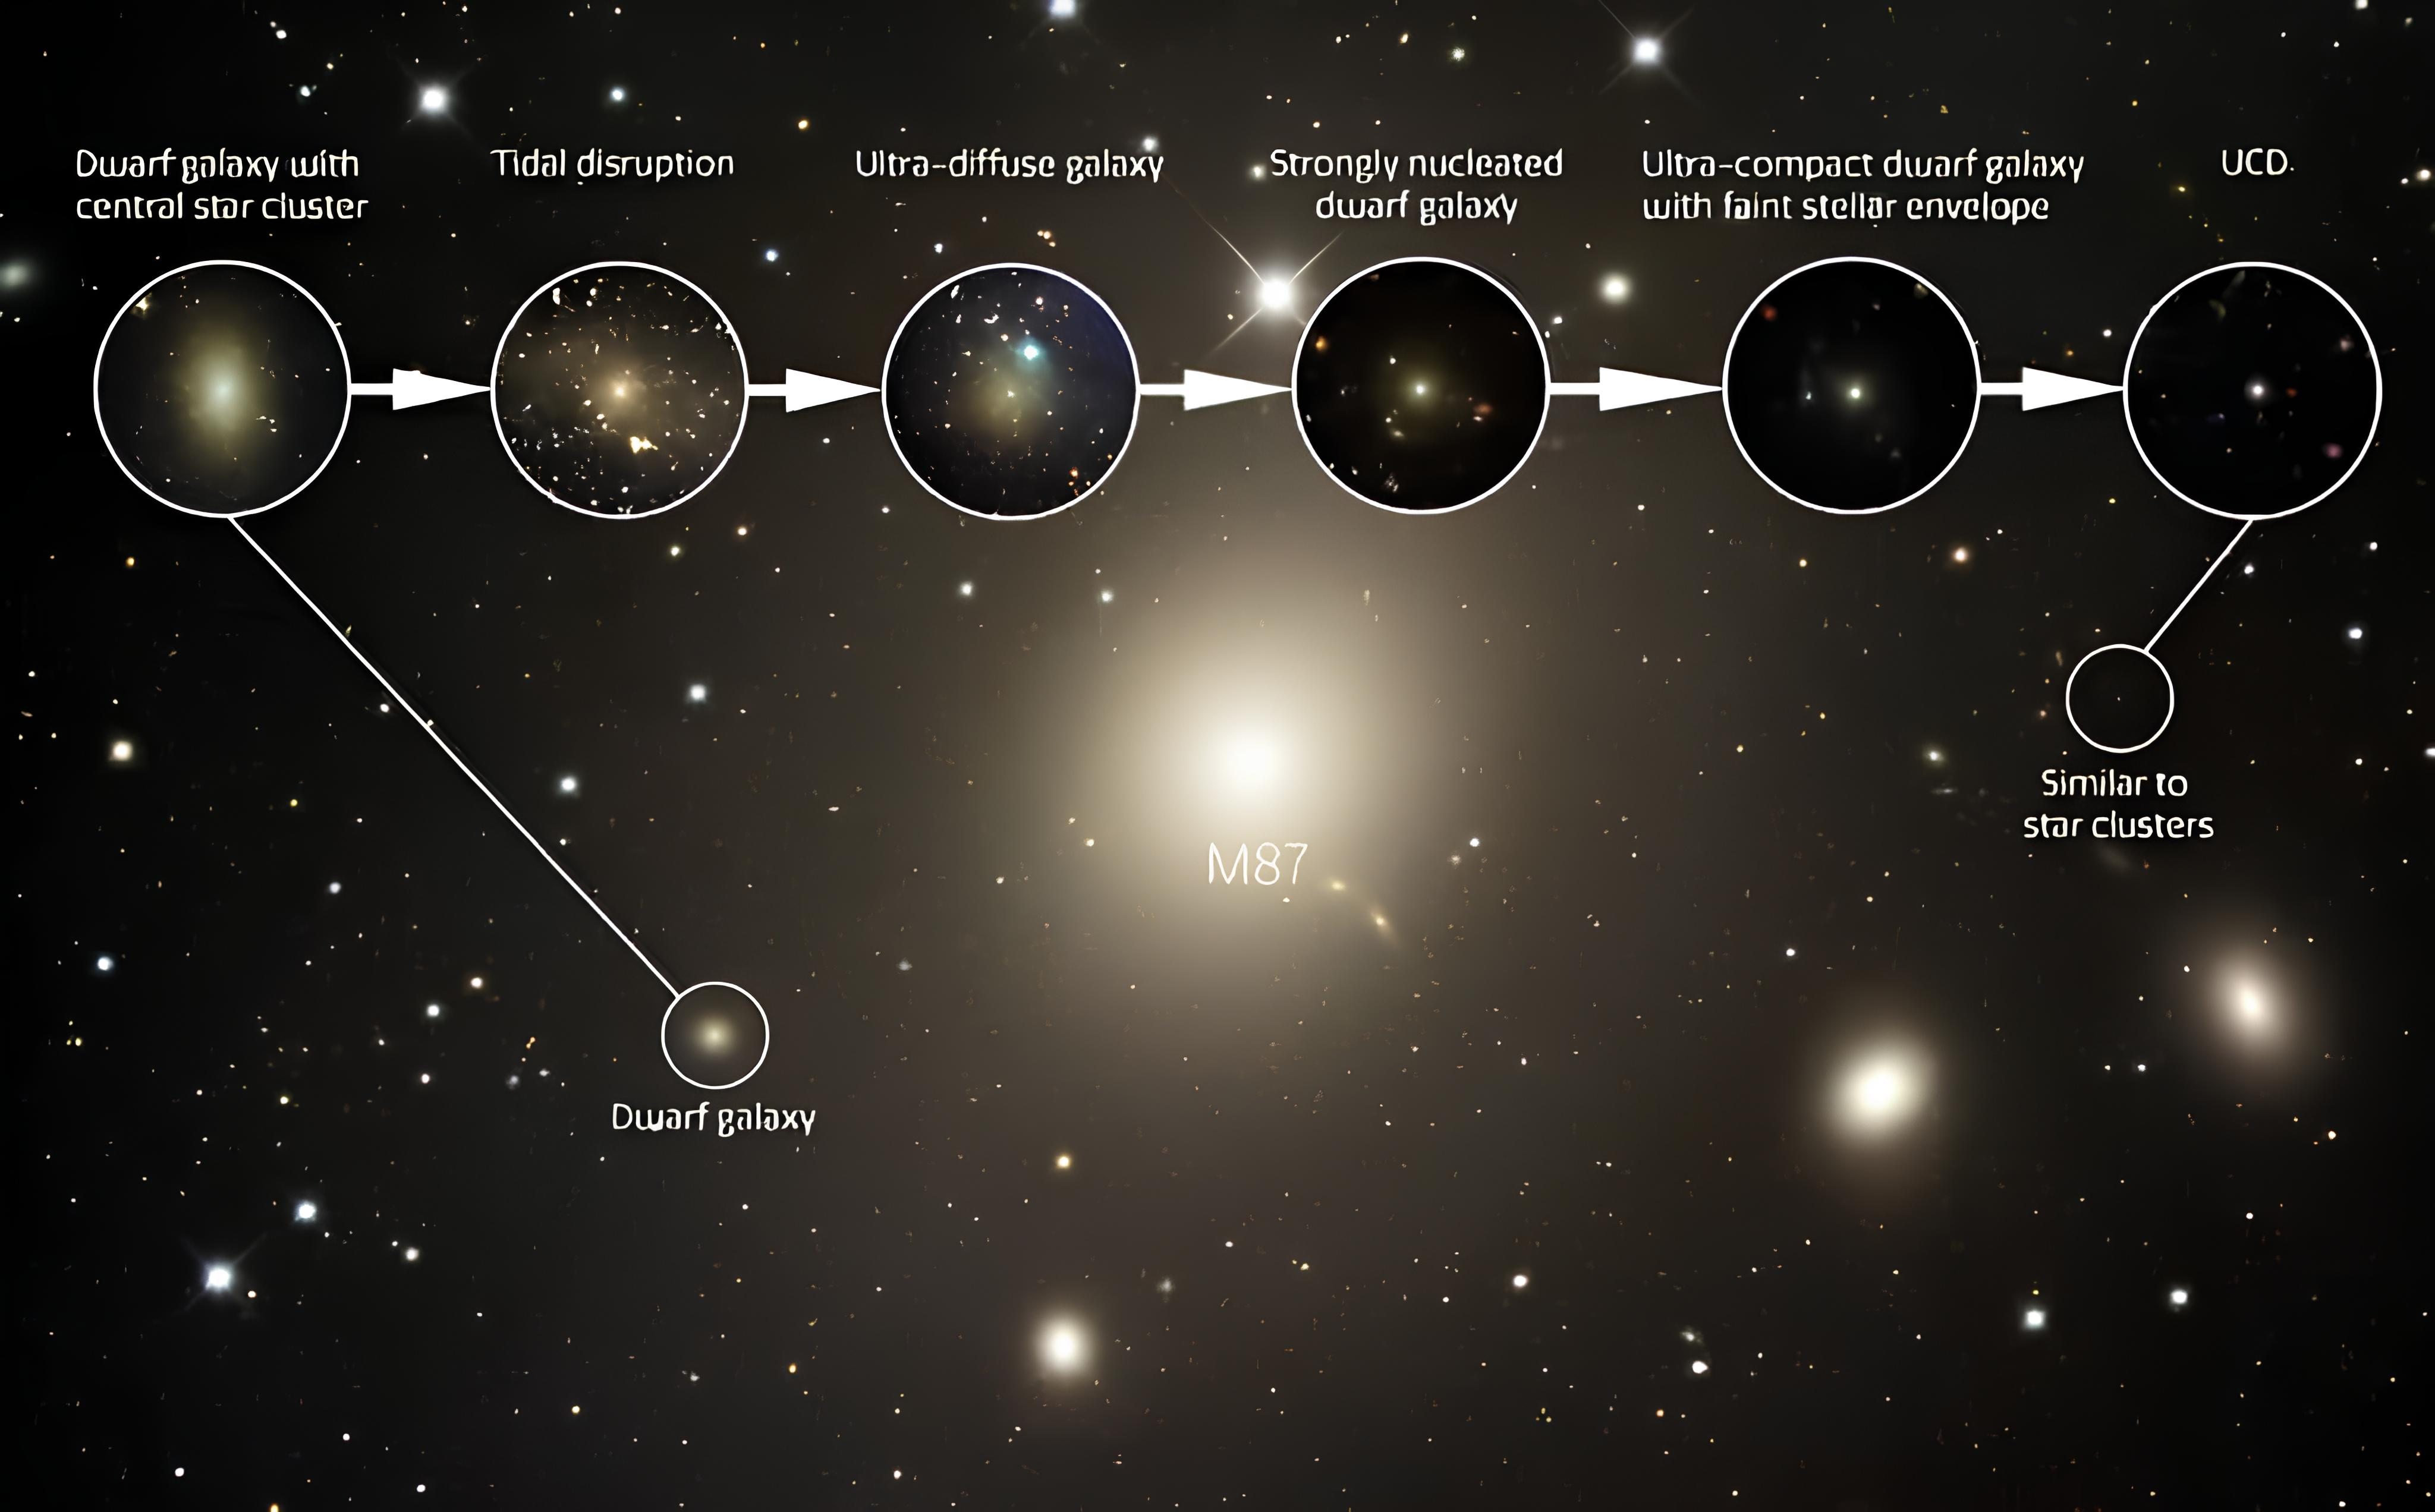
\includegraphics[width=1.\columnwidth,angle=0]{continuo_evolution_dwarf.png} 
    \caption[]{Um contínuo de galáxias capturadas em diferentes estágios do processo de transformação de uma galáxia anã em uma anã ultra-compacta (UCD) num cenário de remoção da envoltória estelar em torno do núcleo. Esses objetos estão localizados perto da supergigante M87, o membro dominante do vizinho Aglomerado de Virgo. Crédito: NOIRLab/NSF/AURA/NASA/R. Gendler/K. Wang/M. Zamani}
    \label{continuo_evolution_dwarf}
\end{figure}

\subsection{Espectroscopia de UCDs}\label{subsec:espectroscopia}
A espectroscopia de galáxias é uma ferramenta essencial para compreender sua história de formação estelar, bem como sua evolução química e dinâmica interna. No caso das galáxias anãs, a espectroscopia permite determinar as velocidades radiais individuais de estrelas (particularmente no Grupo Local), que, por sua vez, são utilizadas para modelar a distribuição de massa e inferir os perfis de matéria escura.

Estudos observacionais demonstraram que as galáxias anãs ultra-compactas apresentam dispersões de velocidade interna significativamente superiores às dos aglomerados globulares. Por exemplo, \cite{Mieske_2008_1} analisaram 23 UCDs no aglomerado de Fornax e encontraram dispersões centrais variando entre 24 e 37 km/s, valores consideravelmente mais altos do que os típicos dos GCs. Além disso, ao serem plotadas no plano dispersão de velocidade versus magnitude absoluta ($\sigma$–$M_V$), as UCDs, especialmente as mais luminosas ($M_V < -12$), alinham-se mais com a extrapolação da relação de Faber-Jackson, característica de galáxias elípticas, do que com a relação observada para GCs.

A espectroscopia desempenha um papel crucial no estudo da cinemática e dinâmica das UCDs. A dispersão de velocidade interna, obtida a partir de linhas de absorção, permite estimar massas dinâmicas e frações de matéria escura \citep{Chilingarian_2011}. Observações realizadas com o Gemini/GMOS de UCDs no grupo fóssil NGC 1132 confirmaram a presença de seis UCDs com velocidades radiais médias e dispersões de velocidade comparáveis às de grupos de galáxias pobres \citep{Madrid_2013}.

Os espectros das UCDs são dominados por linhas de absorção. Linhas proeminentes, como o tripleto de Ca II, Mg b e Fe, são frequentemente observadas, indicando a presença de estrelas antigas e uma metalicidade relativamente alta. Estudos espectroscópicos, como o realizado por \cite{Mieske_2006}, identificaram uma quebra na distribuição de metalicidade em torno de $M_V \approx -11$ mag, sugerindo diferentes origens para UCDs mais brilhantes em comparação com aglomerados globulares. Esses estudos, baseados em índices espectrais e ajustes de síntese de populações, permitiram reconstruir as histórias de formação das UCDs e distinguir aquelas formadas por galáxias nucleadas despojadas de aglomerados globulares massivos \citep{Mieske_2006}.

As análises de \cite{Mieske_2006} também revelaram que, embora UCDs e aglomerados globulares compartilhem algumas características espectrais, as UCDs tendem a apresentar linhas de absorção mais intensas e larguras de linha maiores. Essas diferenças refletem suas maiores massas e possíveis histórias de formação distintas. Assim, os espectros das UCDs, predominantemente compostos por linhas de absorção, evidenciam populações estelares antigas e enriquecidas em metais, destacando sua complexidade e diversidade evolutiva.

\section{Galáxias compactas com emissão}\label{sec:galaxias_compactas_emissao}
As galáxias anãs ultra-compactas e as galáxias anãs compactas azuis (BCDs) são objetos distintos, com propriedades e cenários de formação diferentes. Durante este trabalho de busca por galáxias compactas, nosso método identificou algumas galáxias que podem ser classificadas como BCDs, as quais são mencionadas no Capítulo \ref{chap:spectra_emission}. Nesta seção, discutiremos brevemente suas características e relevância.

As BCDs são galáxias ricas em gás que passam por intensas explosões de formação estelar, frequentemente envolvendo toda a galáxia. Elas foram identificadas pela primeira vez por \cite{Hardie_1956} e \cite{Zwicky_1961}, que as denominaram galáxias anãs compactas. Anos depois, os trabalhos de \cite{Sargent_1970} destacaram esse tipo de objeto ao mostrar que alguns deles apresentavam espectros semelhantes aos das regiões H II encontradas em galáxias espirais. Esses objetos foram então chamados de regiões H II extragalácticas isoladas. Outra classe de galáxias relacionada também foi identificada: as denominadas Green Peas \citep{Cardamone_2009}. Essas galáxias são caracterizadas por sua aparência compacta e esverdeada em imagens do Sloan Digital Sky Survey (SDSS), devido à forte emissão na linha [O III] $\lambda5007$. Os Green Peas compartilham várias propriedades com as BCDs, como baixa massa, baixa metalicidade e altas taxas de formação estelar, sendo considerados análogos locais de galáxias do universo primordial.

Embora os termos BCDs e galáxias H II sejam frequentemente usados de forma indistinta, eles foram originalmente definidos com base em diferentes critérios observacionais: galáxias H II foram identificadas por suas linhas de emissão fortes e estreitas (e.g., \citealt{Terlevich_1991}), enquanto as BCDs foram selecionadas principalmente por suas cores azuis e alta compacidade. Esses critérios distintos revelam certas diferenças físicas entre os dois tipos de galáxias. As propriedades ópticas das galáxias H II geralmente são dominadas por uma ou poucas regiões H II, e suas explosões de formação estelar tendem a ser mais jovens \citep{Telles_1995}. Assim, nem todas as BCDs podem ser classificadas como galáxias H II, já que apenas uma fração das BCDs é dominada por regiões H II.

Muitos estudos têm se concentrado nas BCDs devido às suas características que assemelham-se às de galáxias com alto desvio para o vermelho, tornando-as análogas locais de galáxias do universo primordial \citep{Papaderos_2006}. Inicialmente, acreditava-se que essas galáxias estivessem passando por suas primeiras explosões de formação estelar \citep{Searle_1973, Aloisi_1999, Thuan_1999}, o que as torna objetos de grande interesse para compreender o universo em seus estágios iniciais.

As BCDs apresentam espectros semelhantes às regiões H II de galáxias espirais, embora sejam opticamente pequenas e de baixa luminosidade \citep{Thuan_Martin_1981}. Essas galáxias tipicamente exibem metalicidades subsolares, com [Fe/H] < -1 \citep{Drozdovsky_Tikhonov_2000, Drozdovsky_2001}. A baixa metalicidade, aliada às altas taxas de formação estelar, levanta a questão de saber se esses objetos são realmente jovens ou se estão passando por um surto recente em uma galáxia mais antiga.

Evidências como envoltórios estendidos e avermelhados ao redor das regiões de formação estelar \citep{Loose_1985, Kunth_1985}, bem como perfis de brilho ajustados por leis exponenciais \citep{James_1994, Telles_1995, Papaderos_1996, Cairos_1998}, sugerem que essas galáxias possuem populações estelares antigas, indicando uma história evolutiva mais complexa.

A formação estelar nessas galáxias geralmente ocorre em surtos, mas os mecanismos que desencadeiam o primeiro surto ainda não são completamente compreendidos. Diversos processos têm sido propostos, incluindo fusões de galáxias, encontros gravitacionais de passagem e turbulência no gás interestelar \citep{Noeske_2001, Pustilnik_2001, Bekki_2008}. \cite{Watts_2016} realizaram simulações numéricas para investigar as curvas de rotação acentuadas frequentemente observadas em BCDs. Os resultados indicam que, durante a fusão de galáxias anãs irregulares ricas em gás, o gás tende a se concentrar no núcleo da galáxia resultante, aumentando a densidade central em até seis vezes em relação às galáxias progenitoras. Essa concentração de gás no centro não apenas altera a dinâmica interna, mas também desencadeia intensos surtos de formação estelar, resultando em uma alta luminosidade superficial central, uma característica marcante das BCDs.


Observações de conchas estelares, núcleos cinematicamente desacoplados e correntes de maré ao redor de galáxias anãs têm sido interpretadas como vestígios de fusões passadas \citep{Geha_2005, Rich_2012, Penny_2012, Toloba_2014, Daya_2022}. Em muitos casos, a própria distribuição de gás nas BCDs assemelha-se à de remanescentes de fusão, com braços assimétricos e acúmulos irregulares \citep{Ekta_2008}. A presença de companheiras gasosas próximas reforça a ideia de encontros de passagem ou fusões diretas como gatilhos dos surtos de formação estelar \citep{Pustilnik_2001}. Um exemplo notável é o de \cite{Pak_2016}, que identificou uma fusão em andamento de duas regiões azuis com perfis de brilho exponenciais. Esses achados corroboram estudos anteriores que já apontavam as fusões de anãs como mecanismo-chave na origem das BCDs \citep{Noeske_2001, Ostlin_2001, Bekki_2008}, mostrando como o rearranjo dinâmico do gás durante esses eventos molda tanto os surtos de formação estelar quanto as propriedades estruturais dessas galáxias.

Os espectros das BCDs são dominados por linhas de emissão, como H$\alpha$, H$\beta$, [OIII]$\lambda \lambda 4959,5007$, [O II] $\lambda \lambda 3727,3729$, [N II] $\lambda \lambda 6548, 6584$ e [S II] $\lambda 6717$, que refletem a presença de regiões H II ionizadas por estrelas jovens e massivas. Além disso, estudos no infravermelho próximo revelaram linhas de emissão de hidrogênio molecular (H$2$), hélio e ferro, sugerindo processos adicionais, como excitação fluorescente e choques \citep{Izotov_2011}. Em alguns casos, a presença de linhas de emissão largas pode ser atribuída a ventos estelares, supernovas ou, raramente, à atividade de núcleos galácticos ativos \citep{Izotov_2007}.

Modelos de evolução química propõem que as BCDs podem experimentar regimes de formação estelar contínua ou intermitente (\textit{bursting} ou \textit{gasping}). No cenário intermitente, períodos de formação estelar ativa são separados por intervalos de inatividade mais curtos que os períodos ativos. Esses modelos, que consideram uma eficiência moderada de formação estelar e ventos galácticos enriquecidos em metais, conseguem reproduzir as abundâncias químicas observadas em BCDs \citep{Yin_2011}.

Portanto, a formação e evolução das BCDs são influenciadas por uma combinação de processos, como fusões de galáxias anãs, interações em ambientes densos e diferentes regimes de formação estelar. Enquanto as UCDs apresentam espectros dominados por linhas de absorção, refletindo populações estelares antigas e inativas em termos de formação estelar, as BCDs exibem espectros ricos em linhas de emissão, evidenciando formação estelar ativa e recente. Essa distinção espectral destaca os diferentes estágios evolutivos e mecanismos de formação entre esses dois tipos de galáxias.

\section{Plano da dissertação}\label{sec:plano_dissertacao}\label{sec:plano_dissertacao}
Nesta dissertação, buscamos identificar novas galáxias anãs ultra-compactas no aglomerado de Fornax, com ênfase em regiões periféricas. Além disso, apresentamos uma busca relacionada a galáxias compactas que exibem sinais de emissão. Nosso objetivo é expandir a amostra desses objetos, especialmente em áreas menos exploradas, e compreender seu papel na formação e evolução de sistemas compactos. Esta dissertação está organizada da seguinte maneira:

\begin{description}
\item[Capítulo \ref{cap:database} – Base de Dados Fotométricos:] Apresenta o levantamento S-PLUS, detalha as 12 bandas fotométricas disponíveis, procedimentos de redução e correção de extinção, e define critérios de qualidade e cortes fotométricos para a seleção de objetos compactos.

\item[Capítulo \ref{cap:analise} – Busca de UCDs na Região de Fornax:] Este capítulo aborda a busca por galáxias anãs ultra-compactas no aglomerado de Fornax. Inicialmente, apresentamos uma compilação das UCDs conhecidas na literatura e comparamos essas informações com a amostra obtida pelo levantamento S-PLUS. Em seguida, detalhamos o uso de técnicas de aprendizado de máquina, incluindo a construção da amostra de treino, o tratamento de valores e o treinamento de classificadores, para identificar possíveis candidatas. Também discutimos a estimativa de redshifts fotométricos (photo-\textit{z}) e, por fim, descrevemos os critérios de seleção, os cortes morfológicos aplicados e a análise da distribuição espacial das candidatas selecionadas.

\item[Capítulo \ref{chap:spectra_emission} – Objetos Compactos com Emissão:] Este capítulo explora a identificação de objetos compactos que apresentam emissão, com foco em galáxias compactas detectadas no filtro $J0660$. Inicialmente, discutimos os critérios fotométricos utilizados para a seleção desses objetos. Em seguida, detalhamos as observações espectroscópicas realizadas com o telescópio Gemini-S, incluindo o planejamento e a execução das exposições. Também abordamos os procedimentos de redução e análise dos dados espectroscópicos, com ênfase na extração de redshifts e na identificação de linhas de emissão. Por fim, apresentamos uma extensão do método para a busca de novas candidatas a galáxias compactas com emissão, ampliando a amostra inicial.

\item[Capítulo \ref{chap:conclusions} – Conclusões e Perspectivas Futuras:] Sintetiza os resultados, discute o impacto de encontrar UCDs em regiões periféricas para os cenários de formação e propõe linhas futuras, incluindo estudos dinâmicos e simulações hidrodinâmicas.

\end{description}



















% \section{Questões em aberto}\label{sec:Questoes_abertas}

% Embora os estudos sobre as UCDs tenham avançado significativamente nos últimos anos, sua origem e evolução ainda são temas de intenso debate. Diversos cenários foram propostos para explicar sua formação, sendo o stripping tidal de galáxias anãs um dos mais aceitos. No entanto, os modelos clássicos de stripping frequentemente negligenciam o papel das fusões hierárquicas em ambientes de aglomerados, onde pequenas subestruturas podem contribuir para a população final de UCDs. 




% Além disso, abordagens semi-analíticas, apesar de fornecerem insights valiosos, carecem de um tratamento adequado da componente bariônica, que influencia diretamente os processos dinâmicos e os tempos de stripping.

% Diante dessas limitações, as simulações hidrodinâmicas cosmológicas emergem como uma ferramenta essencial para investigar a formação e a distribuição das UCDs no contexto da evolução das galáxias em aglomerados. Essas simulações permitem obter previsões mais robustas sobre a frequência de núcleos despojados e a relação entre UCDs e seus progenitores. Neste capítulo, discutimos algumas das principais questões em aberto sobre a natureza das UCDs e os desafios que permanecem para a compreensão de sua formação e evolução.



